\documentclass[conference]{IEEEtran}

\usepackage{cite}
\usepackage{amsmath,amssymb,amsfonts}
\usepackage{algorithmic}
\usepackage{graphicx}
\usepackage{textcomp}
\usepackage{xcolor}
\usepackage{hyperref}
\usepackage{multirow}
\usepackage{graphicx}
\usepackage{subcaption}
\usepackage{booktabs}
\def\BibTeX{{\rm B\kern-.05em{\sc i\kern-.025em b}\kern-.08em
    T\kern-.1667em\lower.7ex\hbox{E}\kern-.125emX}}

\hypersetup{
	colorlinks=true,
	linkcolor=black,
	filecolor=black,      
	urlcolor=black,
	citecolor=black
}
\begin{document}

\title{The Severity-Infrastructure Paradox: Spatial and Temporal Risk Profiles in Orange County, FL}

\author{\IEEEauthorblockN{TBD}
	\IEEEauthorblockA{\textit{dept. of Statistics \& Data Science} \\
		\textit{University of Central Florida}\\
		Orlando, United States of America \\
		TBD}}

\maketitle
\renewcommand{\abstractname}{Summary}
\begin{abstract}
Traffic safety is an emergent property resulting from the complex, non-linear friction between drivers and their environment. This study moves beyond univariate analysis to investigate the ``Severity-Infrastructure Paradox" in Orange County, Florida, using a dataset of 140,860 observations. By applying an unsupervised DBSCAN (Density-Based Spatial Clustering of Applications with Noise) framework, the research isolates 652 high-density ``Black Spot" clusters to determine if accident severity is driven by physical roadway engineering or situational ``meta-aspects".
\end{abstract}

\section{\textbf{Introduction}}

Traffic safety is an emergent property resulting from the non-linear friction between drivers and their environment.

This report moves beyond univariate analysis to investigate whether accident severity correlates directly with roadway infrastructure or is driven by meta-aspects—the complex interplay of temporal, environmental, and situational variables.  

Utilizing a refined dataset for Orange County, Florida, this study applies the DBSCAN unsupervised learning framework to pinpoint high-density ``Black Spots" while isolating random noise. 

By evaluating these spatial clusters, the analysis distinguishes whether high-risk zones are products of infrastructure failure or broader, systemic meta-factors.

\subsection{\textbf{Dataset Structure}}
\indent Derived from \cite{moosavi2019countrywide}, \cite{moosavi2019accident}, and \cite{fdot_geospatial}, the dataset was procured via streaming APIs from the US Department of Transportation and law enforcement agencies. For this analysis, the data was narrowed to 140,860 Florida-specific observations.\\
\indent The structure incorporates 46 multidimensional features—including numeric environmental metrics (e.g., \texttt{Temperature(F)}, \texttt{Visibility(mi)}), categorical weather descriptors, and boolean road attributes (e.g., \texttt{Junction}, \texttt{Traffic\_Signal})—providing the necessary framework for unsupervised cluster analysis.

\vspace{2mm}

\section{\textbf{Methods}}

\subsection{\textbf{Data Preprocessing}}
Data preprocessing was kept minimal to preserve the integrity of the raw observations, involving little more than the removal of non-relevant features. The dataset was refined from an initial 46 variables down to 19, focusing primarily on infrastructure characteristics, spatial coordinates, and temporal markers.\\
\indent This targeted feature set ensures that the clustering model prioritizes physical roadway design and situational context when identifying high-density accident locations.

\subsubsection*{\textbf{Normalization}}
\indent Following feature engineering of temporal variables and the conversion of logical indicators into binary format, the analysis performed a zero-variance check to drop columns providing no discriminative power.\\
\indent The remaining features underwent \textbf{Z-score Normalization} \cite{ISLR2} (zero mean, unit variance) to ensure feature magnitude did not bias subsequent clustering algorithm.

\vspace{2mm}

\subsection{\textbf{Exploratory Data Analysis (EDA)}}
With the dataset stabilized and standardized, the exploratory analysis focused on uncovering the underlying environmental and temporal patterns that characterize Orange County's traffic risk.

\subsubsection*{\textbf{Infrastructure Trends}}

Within the infrastructure space, analysis of Figure \ref{plot_severity_infrastructure}, reveals that Crossings serve as the primary hotspot for accidents, with a sharp peak at Severity \textbf{Level 2}.

\begin{figure}[htbp]
	\centerline{
\includegraphics[scale=0.30]{plot_severity_infrastructure.pdf}}
	\caption{Infrastructure Patterns Distribution}
	\label{plot_severity_infrastructure}
\end{figure} 

While Traffic Signals and Stations show elevated incident counts at this same severity level, their impact remains secondary to that of crossings.\\
\indent Notably, Junctions exhibit a much lower accident density across the board, suggesting that in this specific data environment, pedestrian or road crossings pose a higher safety risk than traditional network nodes.

\begin{table}[h]
	\centering
	\begin{tabular}{|l|c|c|c|c|}
		\hline
		\textbf{Infrastructure Type} & \textbf{Sev 1} & \textbf{Sev 2} & \textbf{Sev 3} & \textbf{Sev 4} \\ \hline
		Crossing & Low & High & Med & Low \\ \hline
		Junction & Low & Med-Low & Low & Low \\ \hline
		Traffic Signal & Low & Med & Low & Low \\ \hline
		Station & Low & Med-Low & Low & Low \\ \hline
	\end{tabular}
	\caption{Simplified Accident Severity Heatmap Data}
	\label{tab:accidents}
\end{table}

\subsubsection*{\textbf{Temporal and Distributional Trends}} 

Figure \ref{plot_temporal_hour} reveals a strong correlation between peak commuting hours and accident frequency.

\begin{figure}[htbp]
	\centerline{
\includegraphics[scale=0.45]{plot_temporal_hour.pdf}}
	\caption{Hourly Pattern Distribution}
	\label{plot_temporal_hour}
\end{figure} 

A bimodal distribution is evident, with significant spikes occurring during the morning rush (approximately 7:00 AM to 8:00 AM) and a much larger, sustained peak during the afternoon rush hour, reaching its maximum around 4:00 PM to 5:00 PM.\\
\indent Throughout these periods, Severity Level 2 remains the dominant classification, consistently outnumbering more severe incidents.

\begin{figure}[htbp]
	\centerline{
\includegraphics[scale=0.45]{plot_temporal_day.pdf}}
	\caption{Daily Pattern Distribution}
	\label{plot_temporal_day}
\end{figure} 

On a weekly scale (Figure \ref{plot_temporal_day}), accident volume remains high and relatively stable during the workweek (Monday through Friday), with Friday exhibiting the highest total incident count.\\
\indent Conversely, there is a substantial drop in total accidents during the weekend, particularly on Sunday, which records the lowest volume in the dataset.\\
\indent Despite these fluctuations in total volume, the proportion of different severity levels appears to remain largely consistent across all days.

\subsubsection*{\textbf{Infrastructure and Crash Severity Summary}}

\textbf{Crash Severity Index (CSI) \cite{LiBai2008}:} A weighted metric used to prioritize high-impact accidents over raw frequency. In this dataset, the \textbf{Avg. CSI is 2.0958}.\\
\indent It is essential for identifying whether specific infrastructure nodes are suffering from systemic safety failures or are influenced by external \textbf{meta-aspects}.

\noindent \textbf{CSI Summary Statistics:} \\
Total Crashes: 140,860 \quad | \quad Total CSI Score: 295,220 \quad | \quad Avg. CSI per Crash: 2.0958

\begin{table}[h]
	\centering
	\small
	\begin{tabular}{lrr}
		\hline
		\textbf{Infrastructure Feature} & \textbf{Count (N)} & \textbf{Ratio} \\ \hline
		Crossing & 52,700 & 0.3741 \\
		Traffic Signal & 30,031 & 0.2132 \\
		Station & 11,677 & 0.0829 \\
		Junction & 2,771 & 0.0197 \\
		Stop & 1,652 & 0.0117 \\
		Amenity & 712 & 0.0051 \\
		Railway & 594 & 0.0042 \\ \hline
	\end{tabular}
	\caption{Top Infrastructure Features by Crash Frequency and Ratio.}
\end{table}

An \textbf{Avg. CSI of 2.0958} is statistically significant as it positions the mean accident severity well above the baseline for minor incidents.\\
\indent This value indicates that infrastructure-related crashes in this dataset are predominantly injury-prone, providing a benchmark to identify outliers where \textbf{meta-aspects}—such as high-speed highway junctions—disproportionately escalate risk.

\vspace{4mm}

\subsubsection*{\textbf{West Orlando Case Study}} 

Spatial analysis (Figure \ref{west_cfl_overview}) reveals accident clusters at \textbf{I-4} and \textbf{408 Expressway} junctions. A color-coded hierarchy is shown to denote severity: blue dots represent \textbf{Level 2} incidents, while green and yellow signify the higher \textbf{Levels} 3 and 4, respectively.

\begin{figure}[htbp]
	\centerline{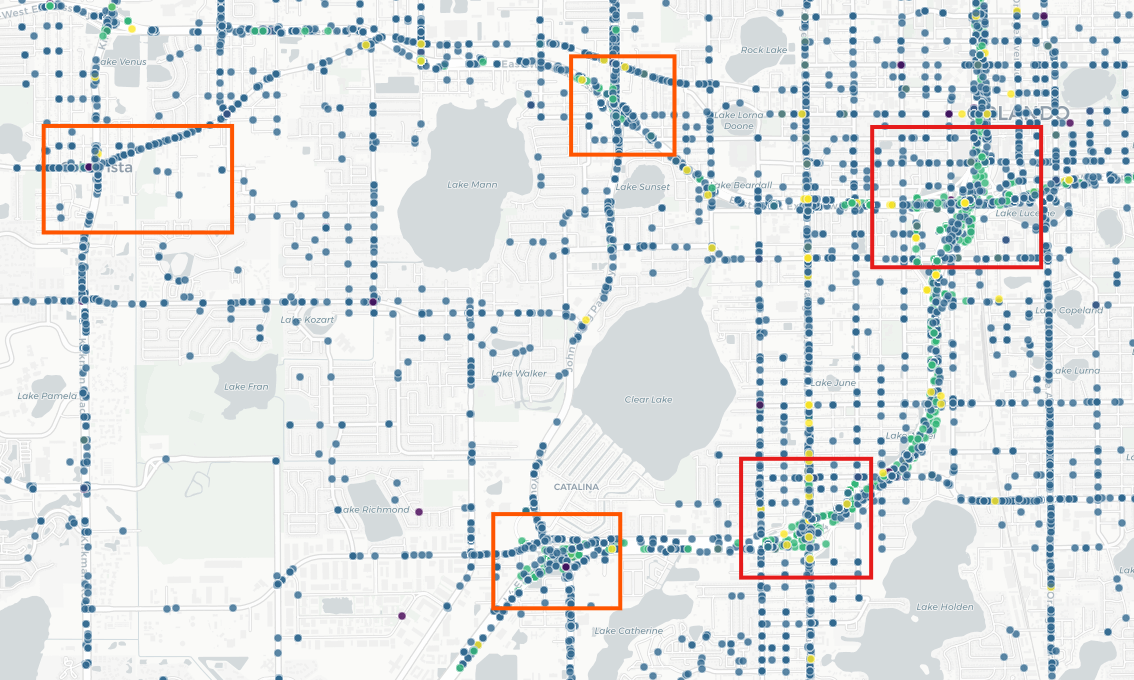
\includegraphics[scale=0.25]{west_cfl_overview.png}}
	\caption{West Orlando Zoomed-In Raw Density}
	\label{west_cfl_overview}
\end{figure} 

This high-density pattern tests the central problem statement: is severity a direct result of roadway infrastructure, or is it driven by \textbf{meta-aspects}—the complex interplay of temporal, environmental, and situational variables that transcend simple engineering?

\vspace{2mm}

\subsection{\textbf{Validation Methodologies}}

This high-density pattern tests whether severity is a direct result of roadway infrastructure or is driven by \textbf{meta-aspects}---the complex interplay of temporal, environmental, and situational variables. To validate the structural integrity of these patterns, we employ metrics specifically designed for density-based algorithms that account for non-spherical shapes and noise:

\begin{itemize}
	\item \textbf{Shadow Silhouette \cite{Maia2017}:} An optimized version of the Silhouette Coefficient, this metric measures the ``certainty" of an observation's placement within a dense core versus its proximity to the ``shadow" (the transition zone into noise), from 1 to -1, where 1 is Perfect. Because DBSCAN allows for arbitrary shapes, Shadow Silhouette provides a more accurate reflection of cluster stability by evaluating core-to-border connectivity.
	
	\item \textbf{Density Contrast Ratio \cite{Volker2024}:} This serves as the primary validator for density-based logic. It computes the ratio of point density within the identified clusters against the density of the surrounding unallocated ``noise" points. A high contrast ratio confirms that the algorithm has successfully isolated significant signals from the background entropy.
\end{itemize}

\indent Due to the $O(N^2)$ complexity of distance-matrix calculations, a stratified random sample of \textbf{10,000} observations was utilized for \textbf{Shadow Silhouette}.

 For a population of $N=140,860$, this sample size is \textbf{statistically significant}, yielding a margin of error of $\pm0.94\%$ at a 95\% confidence interval. This ensures the sample remains a reliable proxy for the global dataset's topological structure while maintaining computational efficiency.


\subsection{\textbf{Clustering Framework }}

To investigate the ``meta-aspects" of accident severity, we utilize \textbf{Density-Based Spatial Clustering of Applications with Noise (DBSCAN)} \cite{Ester1996}.\\
\indent Unlike centroid-based methods, \textbf{DBSCAN} is uniquely suited for spatial accident data because it identifies clusters based on the local density of points, allowing for the discovery of non-linear geographic shapes and—crucially—the filtering of outliers as ``noise". This enables us to isolate high-risk hotspots from the general background of isolated traffic incidents.

\subsubsection*{\textbf{Hyperparameter Selection `The Elbow Method'}}The effectiveness of \textbf{DBSCAN} depends on two parameters: $\epsilon$ (the maximum radius of a neighborhood) and minPts (the minimum number of points required to form a dense region).\\

\begin{figure}[htbp]
	\centerline{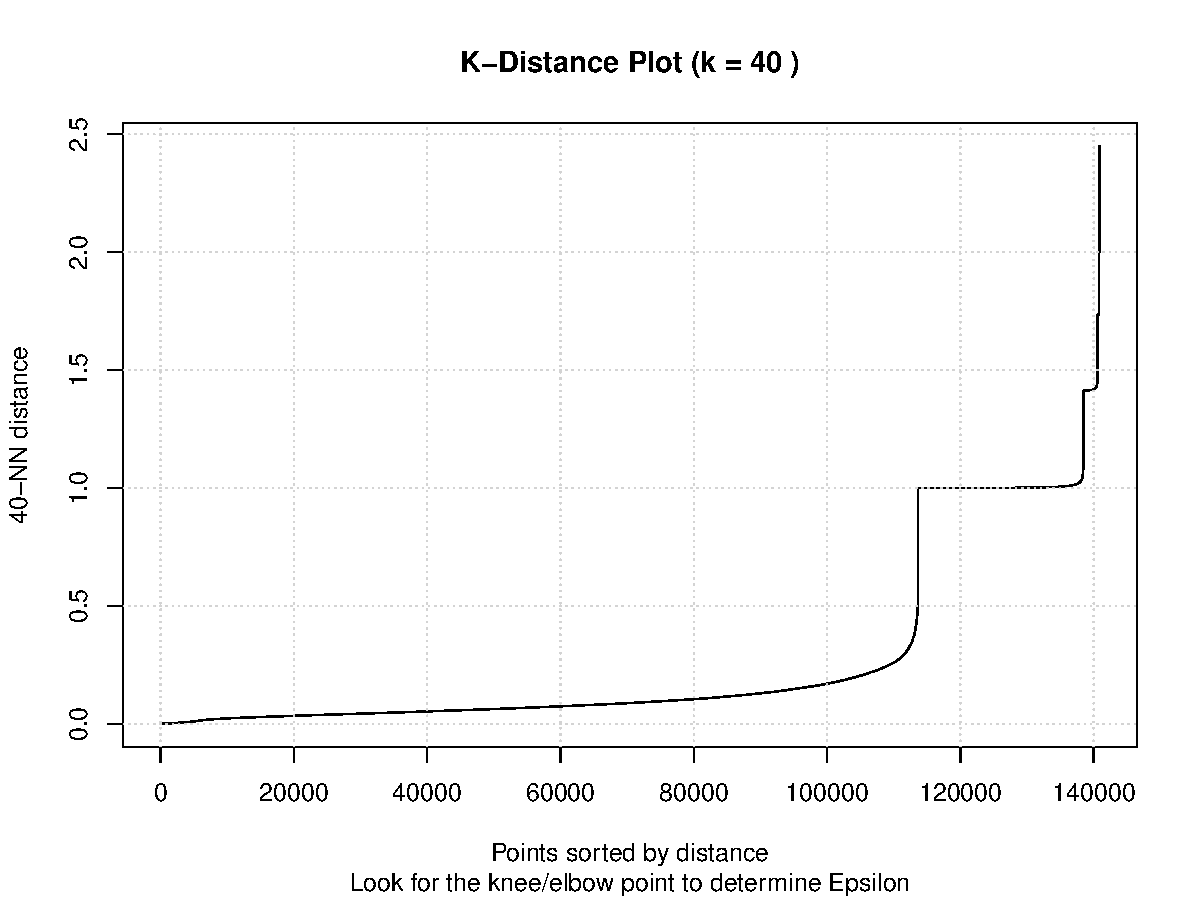
\includegraphics[scale=0.25]{k_distance_elbow.pdf}}
	\caption{K-Distance Plot: Elbow for $\epsilon$}
	\label{k_distance_elbow}
\end{figure} 

To determine the optimal $\epsilon$, we generated a K-Distance Plot (see Figure \ref{k_distance_elbow}).\\
\indent By calculating the distance to the $40^{th}$ nearest neighbor for each of the 140,860 observations and sorting them, we observe a distinct ``elbow" or ``knee" point. This inflection point indicates the threshold where the density begins to drop sharply; per the plot, this occurs at approximately $\epsilon \approx 0.35$. 

\subsubsection*{\textbf{Evaluation of Clustering Trials}} 

With $\epsilon$ fixed at 0.35 based on the k-distance analysis, we conducted three trials varying the minPts threshold (40, 50, and 60) to optimize the balance between cluster granularity and noise reduction. The results of these trials are summarized in Table \ref{table:dbscan_results}.

\begin{table}[h!]
	\centering
	\begin{tabular}{|l|c|c|c|}
		\hline
		\textbf{Metric} & \textbf{Trial 1 (Selected)} & \textbf{Trial 2} & \textbf{Trial 3} \\ \hline
		\textit{minPts} & 40 & 50 & 60 \\ \hline
		Total Clusters & 652 & 573 & 496 \\ \hline
		Noise Points & 26,923 & 30,434 & 34,612 \\ \hline
		Noise Percentage & $\approx$ 19.11\% & $\approx$ 21.61\% & $\approx$ 24.57\% \\ \hline
		Density Contrast Ratio & $\approx$ 11.30 & $\approx$ 10.03 & $\approx$ 9.41 \\ \hline
		Shadow Silhouette Score & $\approx$ 0.8336 & $\approx$ 0.8334 & $\approx$ 0.8316 \\ \hline
	\end{tabular}
	\caption{Comparison of DBSCAN Hyperparameter Trials ($\epsilon \approx 0.35$)}
	\label{dbscan_results}
\end{table}

As shown in Table \ref{dbscan_results}, Trial 1 (minPts = 40) was selected as the optimal framework for several reasons:
\begin{itemize}
	\item \textbf{Superior Density Capture:} It achieved the highest \textbf{Density Contrast Ratio (11.30)}, indicating a more distinct separation between the dense accident cores and the sparse surrounding noise.
	\item \textbf{Metric Stability:} It maintained the highest \textbf{Shadow Silhouette Score (0.8336)}, suggesting the most cohesive internal cluster structure.
	\item \textbf{Granularity:} By keeping the noise percentage at 19.11\%, it preserved a larger portion of the dataset for analysis compared to the more restrictive 50 and 60 minPts trials, which discarded significantly more data as noise (up to 24.57\%).
\end{itemize}  This framework provides the spatial foundation required to test whether these 652 identified clusters exhibit severity patterns linked to engineering or the aforementioned meta-variables.

\vspace{2mm}

\section{\textbf{Experimental Results}}

\subsection{\textbf{Clustering Exploration and Analysis}}

The analysis of top clusters (Table \ref{cluster_analysis}) reveals three distinct risk profiles based on the interaction of frequency, severity, and infrastructure presence.\\
\indent Within this framework, \textbf{Severity}, \textbf{Peak Hour}, and \textbf{Day} are defined as the mean values of all observations within a given cluster for those respective features, representing the central tendency of the cluster's behavior.\\
\indent In contrast, the \textbf{Infrastructure} metric represents the aggregate presence of infrastructure assets, calculated as the summation of all individual infrastructure features—including traffic signals, junctions, crossings, and stations—recorded across the cluster's observations.

\begin{table}[htbp]
	\centering
	\footnotesize
	\setlength{\tabcolsep}{3pt} 
	\begin{tabular}{@{}lccccccl@{}}
		\toprule
		\textbf{Cat.} & \textbf{ID} & \textbf{Freq.} & \textbf{Infra} & \textbf{Sev.} & \textbf{Peak} & \textbf{Day} & \textbf{Score} \\ \midrule
		\textit{Freq.} 
		& 228 & 1,151 & 0 & 2 & 4PM & Tue & 1841.6 \\
		& 320 & 1,146 & 0 & 2 & 5PM & Wed & 1833.6 \\
		& 137 & 1,133 & 0 & 2 & 5PM & Thu & 1812.8 \\
		& 290 & 1,101 & 0 & 2 & 5PM & Tue & 1761.6 \\
		& 150 & 1,092 & 0 & 2 & 4PM & Fri & 1747.2 \\ \midrule
		\textit{Sev.} 
		& 79 & 144 & 0 & 3 & 8AM & Thu & 1.2 \\
		& 181 & 125 & 0 & 3 & 8AM & Tue & 1.2 \\
		& 62 & 124 & 0 & 3 & 8AM & Wed & 1.2 \\
		& 263 & 115 & 0 & 3 & 7AM & Tue & 1.2 \\
		& 57 & 111 & 0 & 3 & 7AM & Wed & 1.2 \\ \midrule
		\textit{Infra} 
		& 7 & 446 & 892 & 2 & 8AM & Thu & 2.2 \\
		& 6 & 386 & 772 & 2 & 7AM & Thu & 2.2 \\
		& 1 & 287 & 574 & 2 & 5PM & Wed & 2.2 \\
		& 9 & 239 & 478 & 2 & 9AM & Thu & 2.2 \\
		& 4 & 120 & 240 & 2 & 8PM & Wed & 2.2 \\ \bottomrule
	\end{tabular}
	\caption{Top Clusters by Frequency, Severity, and Infra}
	\label{cluster_analysis}
\end{table}

\subsection*{1. Frequency-Driven Clusters (High-Volume Peaks)}
These clusters represent the highest operational load, dominated by sheer event volume.

\begin{itemize}
	\item \textbf{Temporal Trend:} Activity peaks consistently during the evening rush hour (\textbf{4:00 PM -- 5:00 PM}), primarily on Tuesday through Thursday.
	\item \textbf{Frequency-Based Priority:} 
	Focuses on high-volume clusters by weighting frequency and total severity.
	\begin{equation}
		P_{freq} = (Frequency \times 0.4) + (Severity_{total} \times 0.6)
	\end{equation}
	\item \textbf{Impact Profile:} While individual severity is moderate (Level 2), the cumulative volume (Freq $> 1,000$) results in the highest overall Priority Scores ($\approx 1800$)
\end{itemize}

\subsection*{2. Severity-Driven Clusters (DBSCAN-Identified Maxima)}
This category identifies dense spatial groupings where DBSCAN determined a 100\% concentration of maximum severity events, visualize in (Figure \ref{Severity_Cluster_Map}).
\begin{itemize}
	\item \textbf{Threshold Consistency:} Unlike frequency-weighted clusters, these represent locations where the recorded severity is \textit{uniformly} at the maximum level (Level 3).
	\item \textbf{Temporal Convergence:} These ``Severity Maxima" clusters peak sharply between \textbf{7:00 AM and 8:00 AM}, suggesting that early morning traffic conditions in these specific coordinates are prone to the most severe outcomes.
	\item \textbf{Infrastructure Absence:} The consistent priority score of 1.2 is a direct result of the formula $(0 \times 0.7) + (3 \times 0.4)$, highlighting a significant gap in infrastructure at these high-risk spatial coordinates.
\end{itemize}

\begin{figure}[htbp]
	\centerline{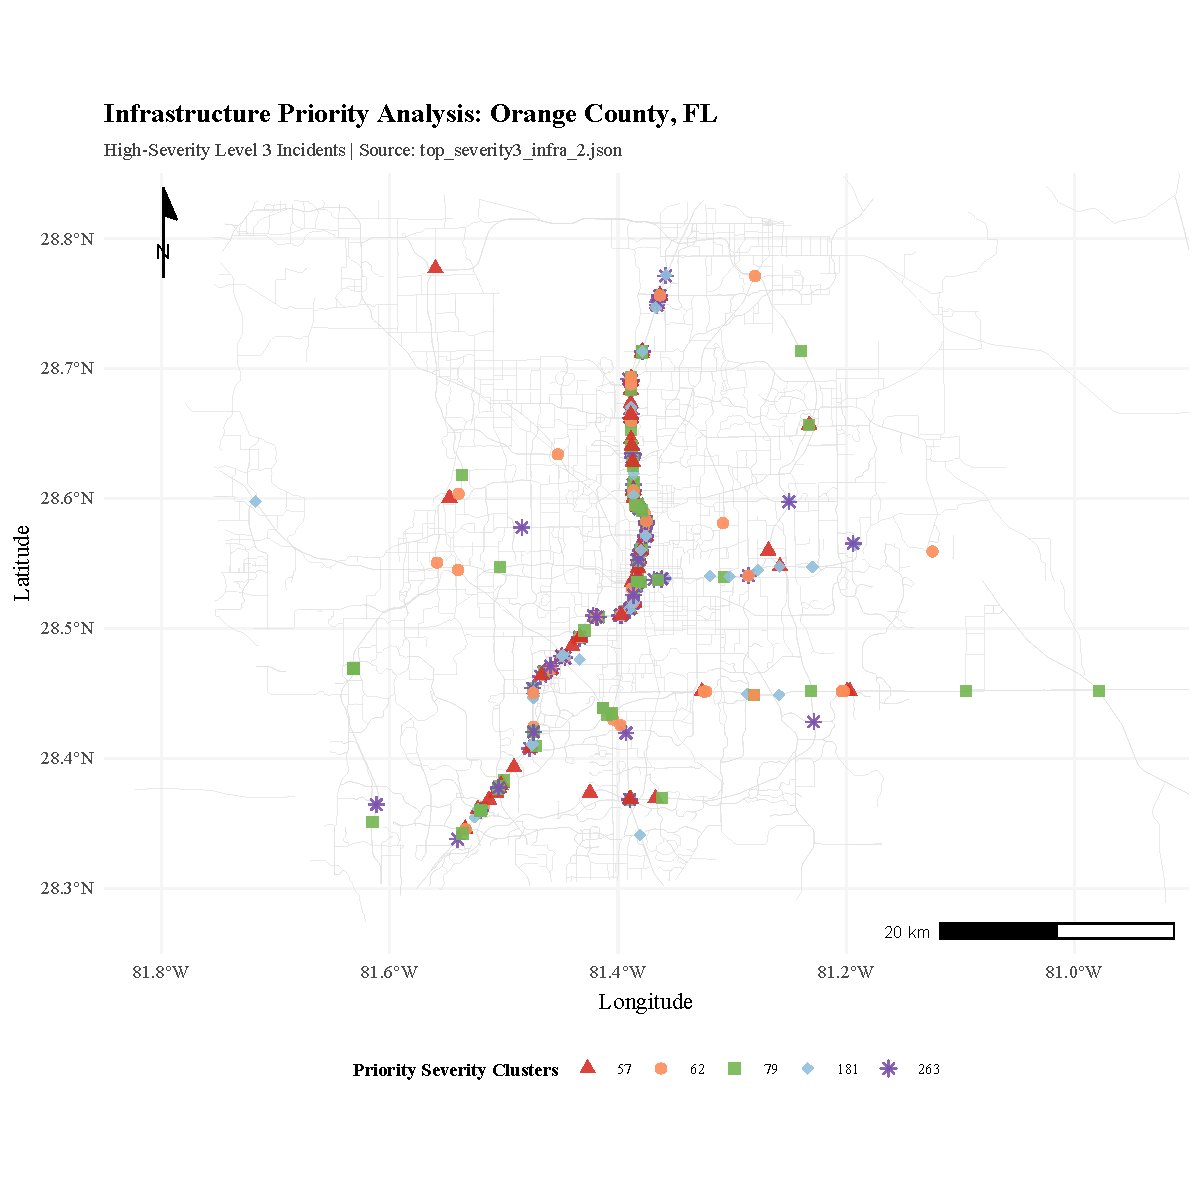
\includegraphics[scale=0.45]{Severity_Cluster_Map.pdf}}
	\caption{Top 5 Severity: I-4 Safety Vacuum}
	\label{Severity_Cluster_Map}
\end{figure} 


\subsection*{3. Infrastructure-Driven Clusters (Asset-Dense Hubs)}
These clusters are defined by high infrastructure presence (weighted at 70\% of the score).

\begin{itemize}
	\item \textbf{Correlation:} There is a fixed ratio between frequency and infrastructure ($Infra = 2 \times Freq$), indicating systematic asset allocation.
	\item \textbf{Operational Window:} Unlike the other categories, these areas show activity across a wider temporal range (\textbf{7:00 AM to 8:00 PM}).
	\item \textbf{Strategy:} Focus on long-term asset maintenance and monitoring of high-density infrastructure zones.
	\item \textbf{Ranking Criteria:} Clusters are ranked by prioritizing infrastructure density ($0.7$ weight) alongside average incident severity ($0.4$ weight):
	\begin{equation*}
		P_{infra} = 0.7(Infra_{pres}) + 0.4(Sev_{avg})
	\end{equation*}
\end{itemize}

\begin{table}[h]
	\centering
	\begin{tabular}{@{}llll@{}}
		\toprule
		\textbf{Profile} & \textbf{Primary Driver} & \textbf{Peak Time} & \textbf{Severity Level} \\ \midrule
		Congestion & Frequency & Late Afternoon & Level 2 (Moderate) \\
		High Risk  & Severity  & Early Morning  & Level 3 (Critical) \\
		Structural & Infra     & All Day        & Level 2 (Moderate) \\ \bottomrule
	\end{tabular}
		\caption{Summary of Regional Risk Profiles}
\end{table}

\section{\textbf{Discussion}}

The analysis identifies a critical ``Safety Vacuum'' along the \textit{I-4 corridor}. While the interstate is designed for unimpeded high-speed transit with standard exits, its inherent lack of regulatory infrastructure—such as traffic signals or junctions that act as natural speed moderators in urban grids—correlates with the highest recorded severity.\\
\indent This suggests that the very features defining a highway (controlled access and high velocity) create a environment where, during the situational pressures of the morning rush, accidents are more likely to escalate to \textbf{Level 3} outcomes compared to infrastructure-dense surface streets.

\subsubsection*{\textbf{1. The Severity-Infrastructure Paradox}}
A stark inverse correlation exists between infrastructure presence and incident lethality. While \textbf{Category 3 (Infrastructure-Driven)} clusters utilize dense assets (up to 892) to maintain moderate \textbf{Level 2} severity, the most critical outcomes occur where engineering is absent.\\
\indent As shown in Figure \ref{Severity_Cluster_Map}, the top \textbf{Level 3} clusters (IDs 79, 181, 62) exhibit \textbf{0\% infrastructure presence}.\\
\indent This suggests that the \textbf{I-4} serves as an unmanaged pipeline where the absence of signals or junctions allows accidents to escalate to maximum severity.

\subsubsection*{\textbf{2. Temporal vs. Volumetric Risk}}
Risk is driven by situational pressure rather than sheer volume.\\
\indent The evening rush (\textbf{4:00 PM -- 5:00 PM}) exhibits the highest frequency but remains at \textbf{Level 2} severity, likely due to natural speed moderation from congestion.\\
\indent Conversely, the \textbf{7:00 AM -- 8:00 AM} window is the exclusive ``danger zone'' for \textbf{Level 3} outcomes.\\
\indent This indicates that the morning professional commute—characterized by high-speed transit on unmanaged segments—creates the county's most lethal conditions.

\subsubsection*{\textbf{3. Systematic Failure of the Commute Grid}}
The data isolates these risks as products of the work-week cycle.\\
\indent Although weekend clusters comprise 28\% of the dataset, none reach the priority thresholds for severity or frequency.\\
\indent The concentration of \textbf{Level 3} events during the weekday morning rush confirms that Orange County's peak risk is a failure of the current infrastructure to mitigate the specific situational pressures of the professional commute on the \textit{I-4 corridor}.

\subsection*{\textbf{Revisiting: West Orlando Case Study}}

The West Orlando corridor serves as the primary evidence for the \textit{Severity-Infrastructure Paradox}.\\
\indent When comparing Figure \ref{Zoom_Map} and Figure \ref{Zoom_Map_Severity}, a clear spatial shift occurs: while frequency clusters are distributed across various surface-street junctions, the severity hotspots consolidate almost exclusively along the \textbf{I-4} unmanaged pipeline.

\vspace{-1.25em}

\begin{figure}[htbp]
	\centerline{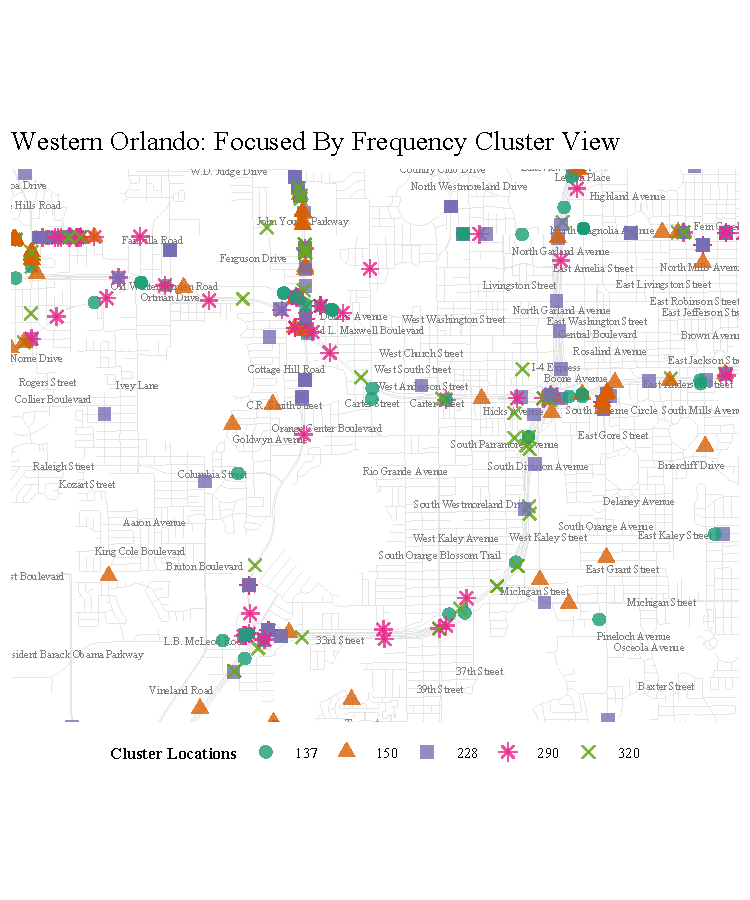
\includegraphics[scale=0.65]{Zoom_Map.pdf}}
	\caption{Top 5 By Frequency: High-volume transit links and weekend activity hubs.}
	\label{Zoom_Map}
\end{figure}  

\begin{figure}[htbp]
	\centerline{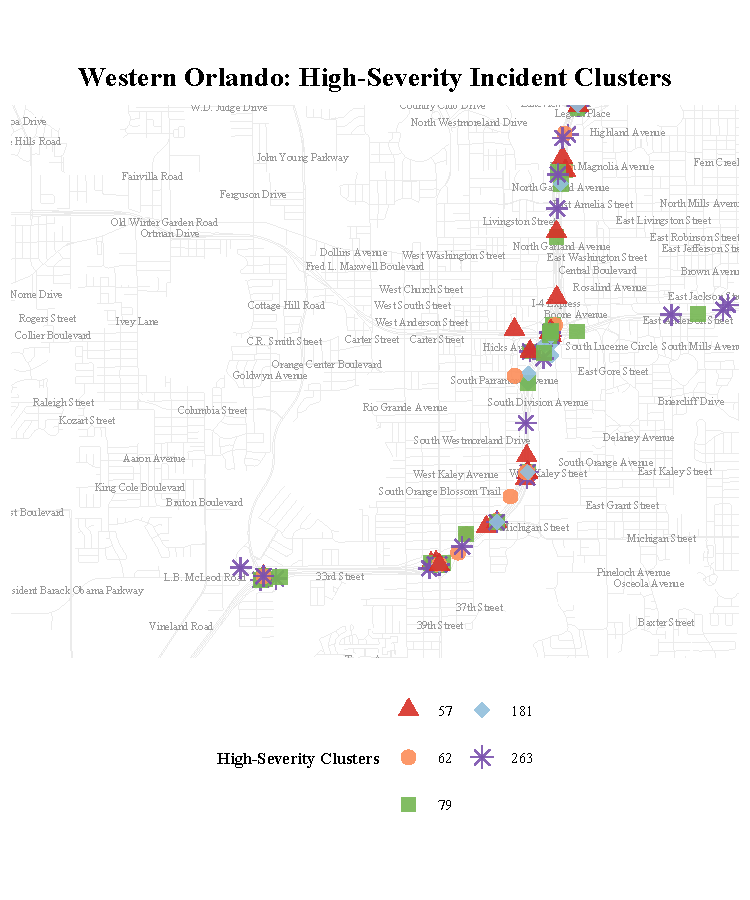
\includegraphics[scale=0.45]{Zoom_Map_Severity.pdf}}
	\caption{Top 5 By Severity: Predominantly ``Low-Infra Priority Areas" along the morning commute risk zone.}
	\label{Zoom_Map_Severity}
\end{figure}

\vspace{.50em}  

This visual transition confirms that risk in West Orlando is not a product of volume, but of situational vulnerability. The morning rush transforms these low-infrastructure segments into ``Early Morning High-Risk" zones, where the absence of regulatory assets allows standard transit conflicts to escalate into \textbf{Level 3} outcomes.


\section{\textbf{Conclusion}}

The analysis of Orange County’s traffic landscape confirms that accident severity is not merely a product of physical engineering, but an \textit{emergent property} of ``meta-aspects"—\textbf{specifically the volatile intersection of temporal pressure and infrastructure absence}. 

While infrastructure-dense zones (e.g., those with signals and crossings) successfully moderate risk to \textbf{Level 2} ``Congestion" profiles, a stark \textit{Severity-Infrastructure Paradox} exists along the \textit{I-4 corridor}.\\
\indent Here, the lack of regulatory assets creates a \textit{``Safety Vacuum"} where the situational pressures of the morning professional commute (7:00 AM – 8:00 AM) escalate standard transit conflicts into critical \textbf{Level 3} outcomes.

\textbf{Ultimately, the data suggests that Orange County’s most lethal environments are driven by situational vulnerability rather than sheer volume}.\\
\indent While the afternoon rush hour produces the highest frequency of incidents, the absence of speed-moderating infrastructure on high-velocity segments during the morning rush remains the primary catalyst for high-severity crashes. 

Addressing these ``Black Spots" requires moving beyond traditional engineering toward \textbf{dynamic, time-sensitive interventions} that account for the systemic friction between the professional work-week cycle and the unmanaged pipeline of the highway system.

\begin{thebibliography}{9}
	
% --- Dataset Requeried ---
	
\bibitem{moosavi2019countrywide}
Moosavi, S., Samavatian, M. H., Parthasarathy, S., \& Ramnath, R. (2019). 
\newblock A Countrywide Traffic Accident Dataset. 
\newblock \textit{arXiv preprint arXiv:1906.05409}.

\bibitem{moosavi2019accident}
Moosavi, S., Samavatian, M. H., Parthasarathy, S., Teodorescu, R., \& Ramnath, R. (2019). 
\newblock Accident Risk Prediction based on Heterogeneous Sparse Data: New Dataset and Insights. 
\newblock In \textit{Proceedings of the 27th ACM SIGSPATIAL International Conference on Advances in Geographic Information Systems} (pp. 33--42). ACM.

\bibitem{fdot_geospatial}
Florida Department of Transportation (FDOT). 
\newblock Florida Geospatial Open Data Portal. 
\newblock \textit{FDOT Transportation Data and Analytics Office}. 
\newblock Available at: \url{https://www.floridagio.gov/maps/} (Accessed: May 2024).

% --- General ---

\bibitem{ISLR2} 
James, G., Witten, D., Hastie, T., and Tibshirani, R. (2021). 
\textit{An Introduction to Statistical Learning: with Applications in R} (2nd ed.). 
Springer Texts in Statistics. New York: Springer.

% --- Infrastructure ---
\bibitem{LiBai2008}
Li, Y. and Bai, Y. (2008).
\textit{Development of Crash-Severity-Index Models for the Measurement of Work Zone Risk Levels}.
Journal of Transportation Engineering, 134(11), 464–474.

% --- Clustering Algorithms ---
\bibitem{Ester1996}
Ester, M., Kriegel, H.-P., Sander, J., and Xu, X. (1996).
\textit{A Density-Based Algorithm for Discovering Clusters in Large Spatial Databases with Noise}.
Proceedings of the Second International Conference on Knowledge Discovery and Data Mining (KDD-96), 226–231.

% --- Evaluation Metrics ---
\bibitem{Maia2017}
Maia, M., and de Carvalho, F. (2017).
\textit{A Modification of the Silhouette Index for the Improvement of Cluster Validity Assessment}.
Proceedings of the International Joint Conference on Neural Networks (IJCNN), 1012–1019.

\bibitem{Volker2024}
Volker, T. B., Gonzalez Poses, C., and van Kesteren, E. J. (2024).
\textit{densityratio: Distribution comparison through density ratio estimation} (Version 0.0.1).
Zenodo. \url{https://doi.org/10.5281/zenodo.13881689}

\section*{\textbf{Appendix}}

\section*{Appendix A: Supplementary Materials and Software Usage}
\subsection*{Source Code Repository \label{app:code}}
The source code, data, and detailed implementation scripts for this project are available on GitHub (URL: \url{https://github.com/gaguillen4384-dev/Data-Science/tree/main/DataMining_2/Risk_Profiles_Car_Accidents_Analysis}).

\subsection*{Software Usage Acknowledgment}
\begin{enumerate}
	\item \textbf{R} (version 4.x.x) was used for model computation and graphics development.
	\item The following \textbf{R} libraries were essential to the computational workflow:
\begin{itemize}
	\item \textbf{data.table}: Utilized for high-performance data manipulation and memory-efficient aggregation of the 140,860-record dataset.
	\item \textbf{dplyr}: Applied for intuitive data piping and grammatical transformations of situational and environmental variables.
	\item \textbf{lubridate}: Used for the precise parsing and extraction of temporal features from crash timestamps.
	\item \textbf{jsonlite}: Employed for the robust ingestion and flattening of nested JSON-formatted traffic data.
	\item \textbf{tidyr}: Used to pivot and reshape the dataset into the tidy formats required for multivariate clustering.
	\item \textbf{ggplot2}: Used as the primary engine for creating all statistical graphics and density plots of crash distributions.
	\item \textbf{leaflet}: Employed to generate interactive spatial visualizations and web-based maps of identified accident clusters.
	\item \textbf{htmlwidgets}: Utilized as a framework to embed interactive JavaScript-based visualizations into the R environment.
	\item \textbf{ggspatial}: Applied to provide specialized spatial data layers and map elements for the analysis of high-density "Black Spots".
	\item \textbf{dbscan}: Utilized for the primary unsupervised learning framework to identify high-density "Black Spots" and spatial accident clusters while effectively isolating random occurrences as noise.
	\item \textbf{tidyverse}: Employed as a meta-package to maintain a consistent data science workflow and dependency ecosystem.
	\item \textbf{sf}: Used for the rapid creation of dummy variables from categorical infrastructure features like signage and junction types.
	\item \textbf{cluster}: Used for basic clustering utilities and the computation of the Silhouette Profile.

\end{itemize}
\end{enumerate}

	
\end{thebibliography}

\vspace{12pt}

\end{document}
